\appendix

\section{Reproduction and Artifact Map}
\label{app:extra}

Every number in this paper is read from a committed JSON artifact or recomputed by a script in the
repository. The main commands are:

{\scriptsize
\begin{verbatim}
python -m bench.v6_audit --ckpt "myna-v5-prototype 2" \
  --split test --every 1 \
  --out runs/paper_v6_audit.json --md runs/paper_v6_audit.md \
  --metrics runs/paper_v6_test.metrics.json \
  --rowout runs/paper_myna_v6_test.rowoutcomes.json
python -m bench.v6_audit --ckpt "myna-v5-prototype 2" \
  --split test --every 1 \
  --max-packed 1000 --out runs/v6_packed_forced.json \
  --rowout runs/v6_packed_forced.rowoutcomes.json
python -m bench.paper_numbers --out runs/paper_numbers.json
python -m bench.consistency_audit \
  --out runs/consistency_audit.json
python -m bench.paper_bootstrap --out runs/paper_bootstrap.json
python -m bench.routing_cost --out runs/routing_cost.json
python -m bench.prob_dump --split test \
  --out runs/v6_prob_test.jsonl
python paper/make_figures_v2.py
\end{verbatim}
}

The routed re-score takes 953 s on CPU for all 1{,}176 bundles and writes all 1{,}440 question
outcomes; the packed-forced arm takes 540 s. \texttt{bench/paper\_numbers.py} recomputes macro,
overall accuracy, joint bundle exact, the per-cell table, per-primitive accuracy, ECE, Brier, and
the risk--coverage curve from those records, and refuses a record whose correctness flag disagrees
with its own prediction and gold. The row-clustered intervals use 20{,}000 bootstrap replicates with
seed 20261104 and resample rows, not questions, because the questions of a bundle share a state.

The witnesses are, one per line:
{\footnotesize\ttfamily\raggedright
runs/paper\_v6\_audit.json \\
runs/paper\_v6\_test.metrics.json \\
runs/paper\_myna\_v6\_test.rowoutcomes.json \\
runs/v6\_packed\_forced.* \\
runs/paper\_numbers.json \\
runs/paper\_bootstrap.json \\
runs/routing\_cost.json \\
runs/consistency\_audit.json \\
runs/paper\_cell\_intervals.json \\
runs/external\_\{majority,tfidf,nli\}.json \\
runs/laya\_0419\_test.rowoutcomes.json \\
runs/vegaml\_0150\_test.rowoutcomes.json \\
runs/latency\_matched.json \\
runs/bench\_mlx\_int8.json \\
runs/browser\_g3.json \\
runs/g6\_* and runs/needle\_* \\
\par}

\paragraph{Known gaps.}
Four training notebooks are in \texttt{release/notebooks/} with their digests: three copies of the
v5 run (training loop, development-split temperature fit, per-option banking77 head, checkpoint
merge) and the v6 run (CAL split, CAL temperature and conformal fit, CORAL gate, checkpoint
assembly). The original CAL file was not committed; the deterministic redraw (1{,}999 bundles,
2{,}548 questions) is now a committed artifact with its SHA-256, and
\texttt{release/build\_cal\_split.py} regenerates it. The suite's committed calibration
split has 448 rows and 568 questions and is a different, earlier split; no number in this paper is
computed from it. The banking77 \texttt{none\_absent}
decomposition is 0/12 here against 7/12 in the training record while the cell aggregate matches at
78/116. These gaps are reported rather than reconstructed.

\section{Per-Cell Results}
\label{app:cells}

Table~\ref{tab:cells} reports the corrected per-cell re-score with row-clustered intervals.

\begin{widetable}
\centering
\footnotesize
\caption{Per-cell corrected re-score with row-clustered 95\% intervals (5{,}000 replicates for the per-cell intervals; 20{,}000 for the macro intervals, seed
20261104). The interval is on the cell accuracy; the unit resampled is the row, not the question.}
\label{tab:cells}
\begin{tabular}{lrrr}
\toprule
Cell & $n$ & Myna & 95\% CI \\
\midrule
agnews/is\_business & 43 & 0.9535 & [0.8837, 1.0000] \\
agnews/is\_scitech & 49 & 0.9184 & [0.8367, 0.9796] \\
agnews/is\_sports & 47 & 0.9787 & [0.9362, 1.0000] \\
agnews/is\_world & 45 & 1.0000 & [1.0000, 1.0000] \\
agnews/topic & 116 & 0.9052 & [0.8448, 0.9569] \\
amazon/stars & 80 & 0.6375 & [0.5250, 0.7375] \\
banking77/intent & 116 & 0.6724 & [0.5862, 0.7500] \\
boolq/answer & 80 & 0.8500 & [0.7750, 0.9250] \\
contrastive/decision & 196 & 0.9847 & [0.9643, 1.0000] \\
dbpedia14/category & 116 & 0.9569 & [0.9138, 0.9914] \\
imdb/positive & 80 & 0.9625 & [0.9125, 1.0000] \\
mnli/relation & 116 & 0.8621 & [0.8017, 0.9224] \\
sst5/sentiment & 80 & 0.6125 & [0.5125, 0.7250] \\
trec/answer\_type & 116 & 0.9483 & [0.9052, 0.9828] \\
yelp/rating & 80 & 0.6250 & [0.5125, 0.7375] \\
yelp/recommend & 80 & 0.9250 & [0.8625, 0.9750] \\
\bottomrule
\end{tabular}
\end{widetable}

The three ordinal cells are the only cells below 0.6, and they are the cells on which the corrected
harness changes the answer. The five agnews boolean cells and the contrastive cell are above 0.95.

\section{Decision Sequence and Diagnostics}
\label{app:sequence}

Figure~\ref{fig:sequence} gives the call sequence for one bundle. The readout is per question; no
cross-question constraint is applied. Figure~\ref{fig:diagnostics} plots the small-engine
diagnostics of Section~\ref{sec:diagnostics}.

\begin{widefigure}
\centering
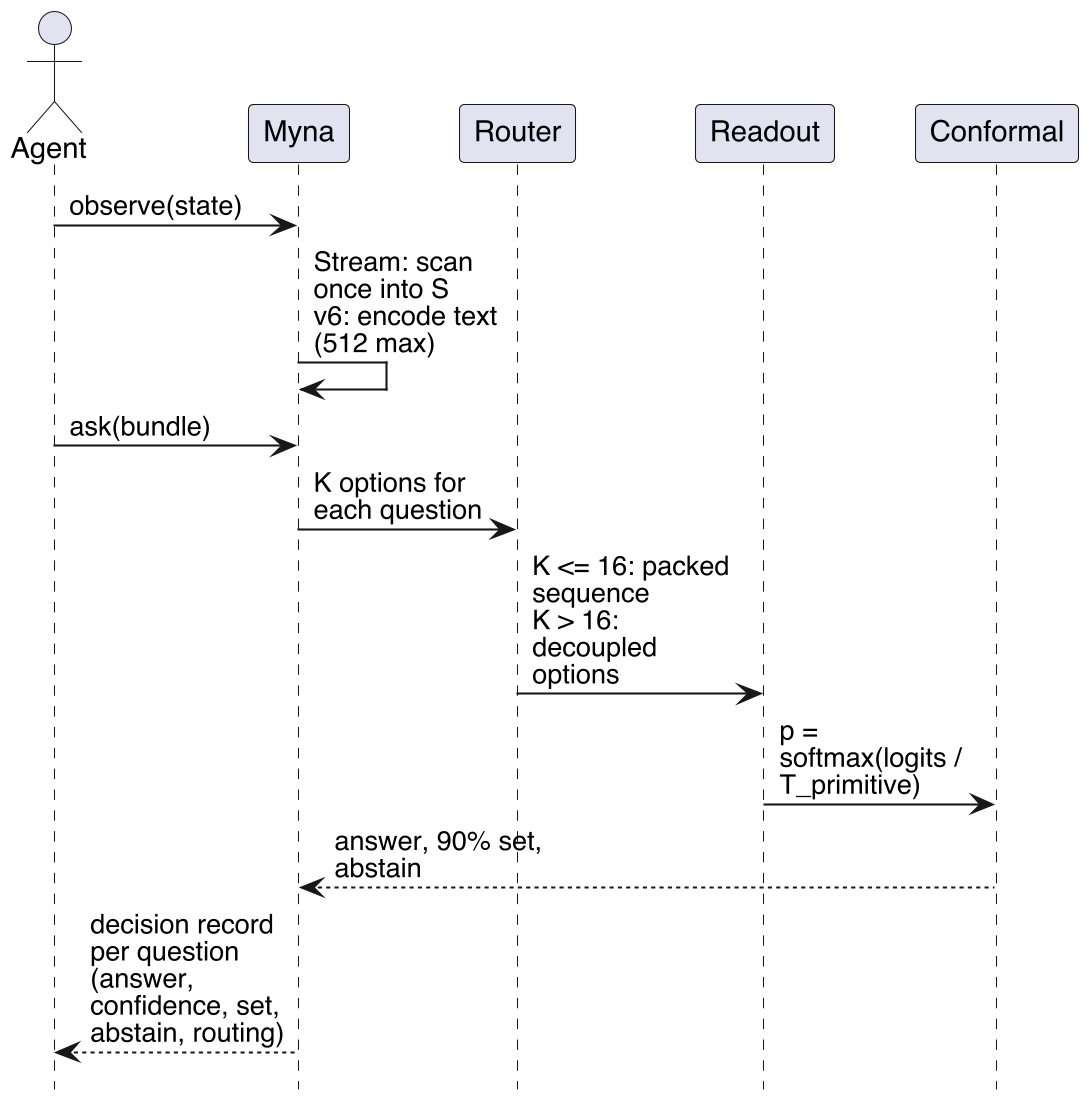
\includegraphics[width=0.72\linewidth]{fig7_sequence.png}
\caption{The \myna{} decision sequence for one bundle. The router chooses packed scoring for
$K\le16$ and decoupled scoring for $K>16$. The conformal gate can attach a 90\% set; this paper
does not use it as a coverage guarantee.}
\label{fig:sequence}
\end{widefigure}

\begin{widefigure}
\centering
\includegraphics[width=0.94\linewidth]{fig6_diagnostics_journal.pdf}
\caption{(a) Synthetic versus real-suite macro for the streaming arms. The dashed line is the 0.94
synthetic gate; the dotted line is the 0.433 majority floor. (b) Needle accuracy against state
length for the 4k-trained arm: flat at the 0.167 uniform floor.}
\label{fig:diagnostics}
\end{widefigure}

\begin{widetable}
\centering
\footnotesize
\caption{Per-cell accuracy on the 1{,}176 test bundles: \vsix{}, the same-backbone per-cell
classifier (seed 21, six epochs, the converged control) and the supervised TF-IDF reference. The
last column is the classifier minus \vsix{}.}
\label{tab:percell_baselines}
\begin{tabular}{lrrrr}
\toprule
Cell & \vsix{} & DeBERTa per-cell & TF-IDF & $\Delta$ (DeBERTa $-$ \vsix{}) \\
\midrule
agnews/is\_business & 0.9535 & 0.9302 & 0.8372 & -0.0233 \\
agnews/is\_scitech & 0.9184 & 0.9796 & 0.8571 & +0.0612 \\
agnews/is\_sports & 0.9787 & 1.0000 & 0.9362 & +0.0213 \\
agnews/is\_world & 1.0000 & 0.9778 & 0.9556 & -0.0222 \\
agnews/topic & 0.9052 & 0.6897 & 0.7931 & -0.2155 \\
amazon/stars & 0.6375 & 0.5625 & 0.5250 & -0.0750 \\
banking77/intent & 0.6724 & 0.6293 & 0.8190 & -0.0431 \\
boolq/answer & 0.8500 & 0.7875 & 0.6125 & -0.0625 \\
contrastive/decision & 0.9847 & 0.8724 & 0.5663 & -0.1122 \\
dbpedia14/category & 0.9569 & 0.7155 & 0.8448 & -0.2414 \\
imdb/positive & 0.9625 & 0.9625 & 0.8500 & +0.0000 \\
mnli/relation & 0.8621 & 0.7155 & 0.4052 & -0.1466 \\
sst5/sentiment & 0.6125 & 0.6250 & 0.3750 & +0.0125 \\
trec/answer\_type & 0.9483 & 0.7414 & 0.7759 & -0.2069 \\
yelp/rating & 0.6250 & 0.5750 & 0.4375 & -0.0500 \\
yelp/recommend & 0.9250 & 0.9250 & 0.7875 & +0.0000 \\
\bottomrule
\end{tabular}
\end{widetable}

